\documentclass[12pt]{article}
\usepackage[utf8]{inputenc}
\usepackage{geometry}
\usepackage{titlesec}
\usepackage{graphicx}
\usepackage{setspace}
\usepackage{times}
\usepackage{footnote}
%\usepackage{natbib}
\usepackage{caption}
\usepackage{float}
\usepackage[titles]{tocloft}
\usepackage{amsmath}
\usepackage{amssymb}
\usepackage{ragged2e} % 添加此宏包用于文本对齐
\usepackage{etoolbox} 
\usepackage{xcolor}
\usepackage{booktabs} % 提供更美观的表格线
\usepackage{siunitx}
\usepackage{makecell}
\usepackage{amsfonts}
\usepackage{listings}
\usepackage{fancyvrb} 
\usepackage[hidelinks]{hyperref}
\usepackage{url} % 用于处理 URL 格式更美观
\usepackage{listings}
\usepackage{xcolor}
\lstset{
    basicstyle=\ttfamily\footnotesize,
    breaklines=true,
    breakatwhitespace=false,
    showstringspaces=false,
    columns=flexible,
    frame=single,
    backgroundcolor=\color{gray!10}
}
\usepackage[
    backend=biber,
    style=ieee,
    sorting=ynt
]{biblatex}
\addbibresource{references.bib}
\renewcommand*{\bibhang}{0pt} % 设置悬挂缩进为 0pt,即去除缩进




% 页边距设置
\geometry{a4paper, left=2cm, right=2cm, top=2.5cm, bottom=2.5cm}
\renewcommand{\familydefault}{\rmdefault}



% 字体与段落格式
\renewcommand{\familydefault}{\rmdefault} % 使用 Roman 字体
\setlength{\parindent}{0pt} % 段落不缩进
\setlength{\parskip}{1em} % 段落间距
\singlespacing % 单倍行距
\justifying % 使用两端对齐

% Section 标题格式优化
\makeatletter
\renewcommand\section{\@startsection{section}{1}{\z@}%
    {-1ex \@plus -0.5ex \@minus -5ex} % 标题前的间距
    {1ex \@plus 0.5ex} % 标题后的间距
    {\normalfont\Large\bfseries}} % 标题字体:正常、加粗、较大
\makeatother

% 标题的字体和大小
\titleformat{\section}[block]{\fontsize{16pt}{18pt}\bfseries}{\thesection}{1em}{}
\titleformat{\subsection}[block]{\fontsize{14pt}{16pt}\bfseries}{\thesubsection}{1em}{}

% 文档开始时设置段落缩进为0
\AtBeginDocument{\setlength{\parindent}{0pt}}

% 定义新命令:设置字体为蓝色 10pt
\newcommand{\tabletext}[1]{\textcolor{blue}{\fontsize{10pt}{12pt}\selectfont #1}}


\newenvironment{Abstract}
{\begin{center}
\section*{Abstract}
\end{center}
\begin{list}{}
    {\setlength{\leftmargin}{5pt}% 左边界设置为0
    \setlength{\parindent}{4em} % 设置段落首行缩进2个汉字宽度(对于英文一般是2em)
    \setstretch{1.8}
    \fontsize{12}{12}\selectfont 
    }}
    {\end{list}}
    
    




\begin{document}

\lstset{
    basicstyle=\ttfamily, % 缩小字体 + 等宽
    breaklines=true,            % 自动换行
    columns=flexible            % 优化对齐
}


% 标题页
\begin{titlepage}
    \centering
    \vspace{0.5cm}
    {\LARGE\bfseries Database - Driven Intelligent Restaurant Management System\par}
    \vspace{0.5cm}
    {\large by \par}
    \vspace{2cm}
    {\large Li Xinze\textsuperscript{1} (2330026083) \par}  
    {\large Li Jiale\textsuperscript{1} (2330026073) \par}  
    {\large Tian Zhiwen\textsuperscript{2} (2230033036)\par}  % Math
    {\large Yan Shan\textsuperscript{2} (2230033048) \par}    % Math 
    \vspace{1.5cm}
    {\large Group 6 Project (COMP3013 Database Management System) \par}
    \vspace{1.5cm}
    {\large Bachelor of Science (Honours) \par}
    \vspace{0.3cm}
    {\large in \par}
    \vspace{0.3cm}
    {\large \textsuperscript{1}Computer Science and Technology\par} 
    {\large \textsuperscript{2}Applied Mathematics \par}      % Math
    \vspace{1.5cm}
    {\large Supervised by\par}
    {\large Dr. Zhijian Li\par}
    \vspace{1cm}
    {\large Beijing Normal University - Hong Kong Baptist University\par}
    {\large \today\par}
\end{titlepage}





\newpage
\tableofcontents

\thispagestyle{empty} 
\pagenumbering{gobble}

% 正文
\newpage

\pagenumbering{arabic} % 设置页码格式为阿拉伯数字
\setcounter{page}{1}

%========================================================
\section{Project Description}

The purpose of this project is to develop a modern restaurant management system that addresses the common real-life challenges faced by restaurants in handling reservations, table allocation, and service coordination. The main problem being solved is the inefficiency and rigidity of traditional restaurant management systems, which make it difficult to track table availability, manage reservations, handle special customer requests, and keep staff updated in real time. This often leads to operational difficulties such as overbooking, underutilization of dining space, delayed service, and poor customer experience.

The difficulty of the problem lies in the need to coordinate multiple moving parts — reservations, table statuses, staff roles, menu management, and real-time updates — within a single system, all while minimizing human error. Additionally, the system must balance usability for both staff and customers, ensure data consistency, and remain adaptable to the dynamic nature of restaurant operations.

Abstractly, this problem can be described as a multi-user, multi-role resource allocation and workflow coordination challenge, where tables are the resources, reservations are the demands, and the system must efficiently match supply to demand in real time. This involves building a robust database with automation, providing intuitive interfaces, and designing a flexible architecture that supports diverse roles and workflows.

The major goal of this project is to create a dynamic, secure, and user-friendly restaurant management platform that streamlines operations, automates routine tasks, and improves the overall efficiency and experience for both staff and customers. By leveraging modern database techniques, automation through triggers, and role-based access control, the system aims to bridge the gap between outdated manual processes and the demands of contemporary restaurant operations.

%========================================================
\section{Our Dataset}
\subsection{Dataset}
The dataset contains synthetic records simulating real-world restaurant data:
\begin{itemize}
    \item Users (customers, receptionists, cleaners, admin)
    \item Tables and table types
    \item Orders with order details
    \item Menu items
    \item Comments/feedback
\end{itemize}

\subsection{Data collection}
Data was generated to cover common restaurant operations, including multiple users with different roles, reservations, cleaning tasks, and menu selections.

\subsection{Data preprocessing approaches}
We cleaned and standardized the data, ensuring consistency in table status, balance amounts, order timestamps, and valid relationships between entities.

%========================================================
\section{Database Design}
\subsection{Assumptions}
\begin{itemize}
    \item Each user has a distinct and exclusive role within the restaurant management system: admin, receptionist, cleaner, or customer. This role-based structure simplifies access control and ensures that users can only perform actions relevant to their job functions.
    \item Each order corresponds to one table, establishing a clear link between the customer's dining experience and the physical seating arrangement. Additionally, each table is assigned to a specific table type, helping with pricing, capacity management, and customer expectations.
    \item Customers can place orders and provide comments. Orders are central to the restaurant's operations, while comments serve as valuable feedback for improvement.
    \item Receptionists manage orders, including taking reservations, updating order statuses, and communicating with customers. Their role ensures a smooth customer experience from booking to meal completion.
    \item Cleaners are responsible for maintaining the cleanliness of dining areas by updating the cleaning status of tables. This ensures that tables are ready for the next customers in a timely manner.
    \item Admins manage table types, including creating new table types, updating their properties (e.g., price, description), and monitoring availability. This flexibility allows the restaurant to adapt to changing business needs and customer demands.
\end{itemize}

\subsection{Entity and Relationship Set}
\subsubsection{Entities}
\begin{itemize}
    \item \textbf{User}: Represents all individuals interacting with the system, storing common information such as uID, name, phone, password, user\_type, and balance. This entity provides a unified framework for managing user accounts and access rights.
    \item \textbf{Admin}: Inherits from the User entity and adds an AdminID to distinguish administrators. Admins have elevated privileges to manage the system, including table types, staff, and settings.
    \item \textbf{Receptionist}: Inherits from the User entity and is identified by Receptionist\_ID. Receptionists manage customer orders, take reservations, and update order statuses.
    \item \textbf{Cleaner}: Inherits from the User entity and is identified by Cleaner\_ID. Cleaners focus on maintaining the cleanliness of tables and updating their clean status.
    \item \textbf{Customer}: Inherits from the User entity and is identified by cID. Customers place orders, make reservations, and provide feedback.
    \item \textbf{Table}: Represents each physical table in the restaurant. It has a unique yID, links to a specific table type (ttID), and records its cleanliness status.
    \item \textbf{Table\_type}: Defines the different table types in the restaurant. It includes ttID, Name, Introduction, Price, Remain, and Img to provide details about each table type for customers and management.
    \item \textbf{Menu}: Stores details about each dish, including dID as the unique identifier, dish name, and price.
    \item \textbf{Order}: Captures each customer order with oID as the unique identifier, linking to the cID of the customer, the tID of the assigned table, the check-in status, the order price, and the order time.
    \item \textbf{Comment}: A weak entity dependent on the order, ensuring that comments are tied to specific orders.
\end{itemize}

\subsubsection{Relationships}
\begin{itemize}
    \item \textbf{User ISA Admin, Receptionist, Cleaner, Customer} \hfill \textit{ISA} \\
        This inheritance relationship models role-based access control. Each user is assigned one role, and common attributes (e.g., name, contact) are stored in the User entity, with role-specific attributes defined in sub-entities.
        
    \item \textbf{Admin Edit Table\_type (admin\_table\_type)} \hfill \textit{(1:N)} \\
        An admin can modify multiple table types, and each table type can be edited by an admin. This relationship supports dynamic configuration of table properties (e.g., capacity, pricing).
        
    \item \textbf{Receptionist Deal Order (receptionist\_order)} \hfill \textit{(1:N)} \\
        A receptionist can handle multiple orders, but each order is processed by exactly one receptionist, ensuring accountability for order management.
        
    \item \textbf{Cleaner Clean Table (cleaner\_table)} \hfill \textit{(M:N)} \\
        Multiple cleaners may be assigned to clean a table, and each cleaner can clean multiple tables, supporting collaborative cleaning schedules.
        
    \item \textbf{Customer Initiate Order (customer\_order)} \hfill \textit{(1:N)} \\
        A customer can place multiple orders, but each order is associated with a single customer. This relationship tracks customer dining history and preferences.
        
    \item \textbf{Table\_type Belong Table (table\_table\_type)} \hfill \textit{(1:N)} \\
        A table type (e.g., VIP, standard) can have multiple instances, but each table belongs to exactly one type. This relationship supports pricing and resource allocation.
        
    \item \textbf{Order Select Menu (orders\_dishes)} \hfill \textit{(M:N)} \\
        An order can include multiple dishes, and each dish can appear in multiple orders. This relationship is modeled via the \texttt{orders\_dishes} associative table, which records the quantity and customization of each dish.
        
    \item \textbf{Order Occupy Table (order\_table)} \hfill \textit{(1:1)} \\
        Each order is assigned to a specific table during the dining period, ensuring exclusive use of the table. This relationship is vital for managing table availability.
        
    \item \textbf{Order Create Comment (order\_comment)} \hfill \textit{(1:1)} \\
        Comments are weak entities dependent on orders. Each comment must reference an existing order, ensuring that feedback is tied to specific dining experiences.
\end{itemize}



\subsection{ER diagram}

\begin{figure}[htbp]
    \centering
    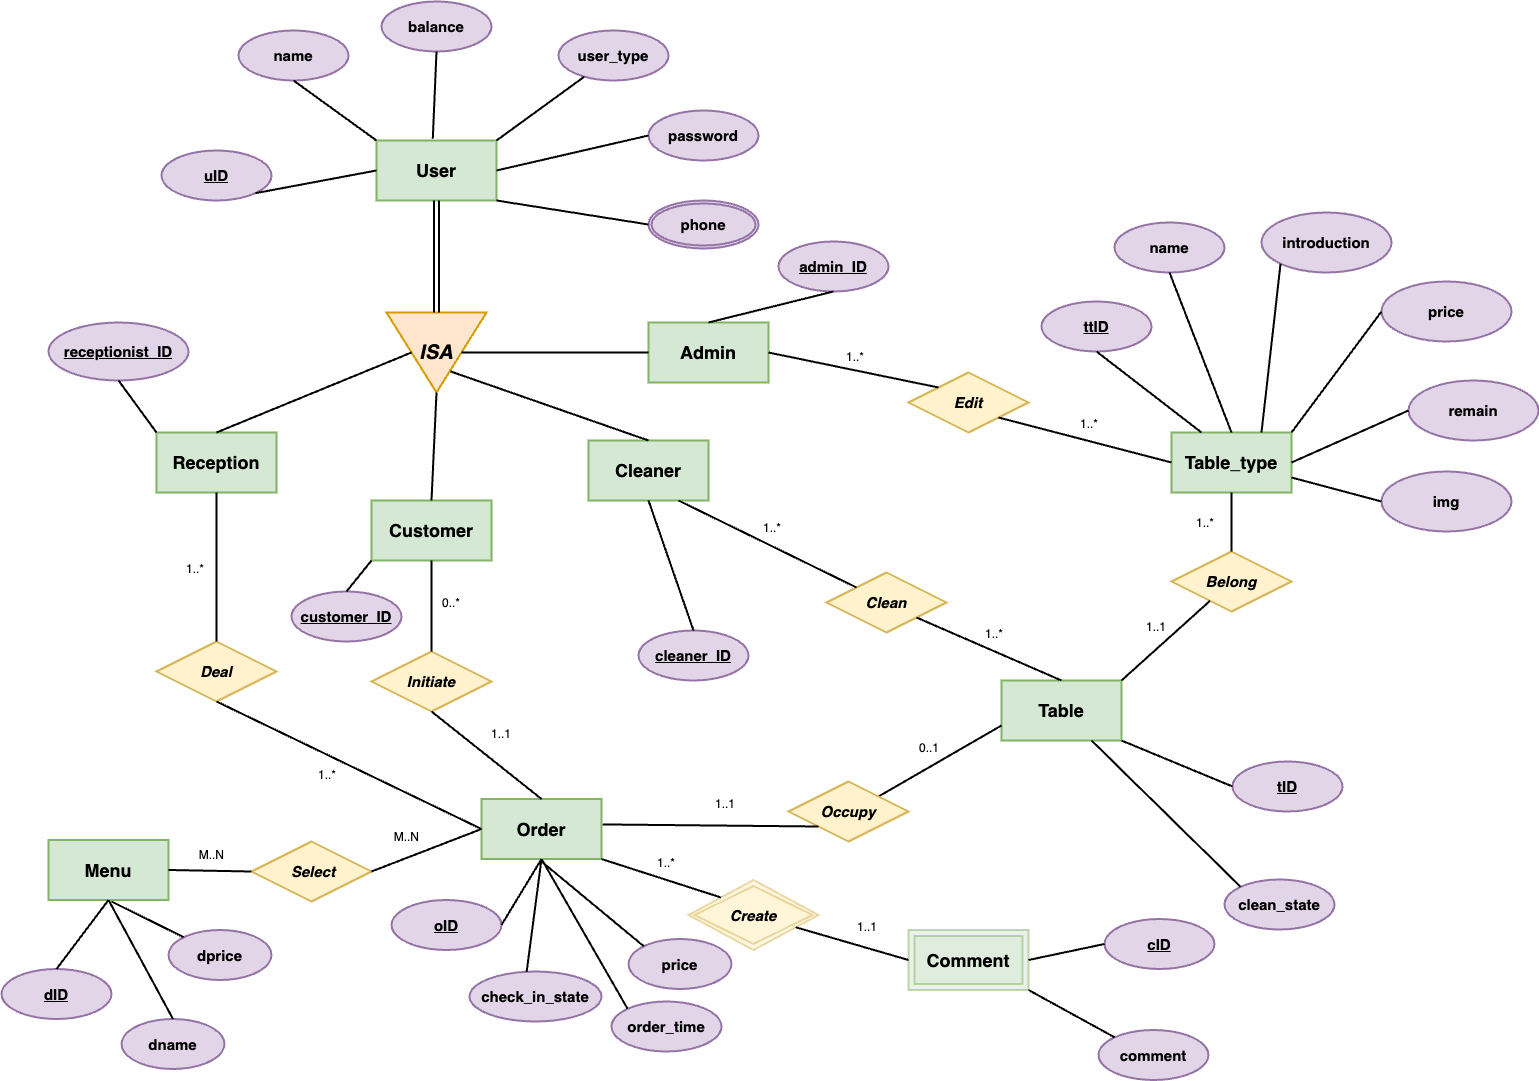
\includegraphics[width=\textwidth]{ER.png} % 这里以示例图片为例,你需要替换为实际的图片文件名
    \caption{ER diagram}
    \label{fig:example}
\end{figure}

The ER diagram visually represents the entities and relationships in the database. At the center is the user entity, with inheritance relationships branching out to admin, receptionist, cleaner, and customer entities, clearly indicating the role - based structure. The table entity is connected to the table type entity through a one - to - many relationship, signifying that multiple tables can belong to the same table type. The order entity acts as a central hub, connecting to the user (customer), table, and menu entities, which effectively reflects the complex interactions during the dining process. The comment entity is linked to the order entity, emphasizing its dependence on the existence of an order.



\subsection{Functional Dependencies}
The following functional dependencies represent the relationships between attributes in the database schema, capturing the rules of attribute determination based on keys:

\begin{itemize}
    \item \( \text{uID} \rightarrow \text{name, phone, , password, user\_type, balance} \)  \\
    For any user (\( \text{uID} \)), the associated name, phone number, user type (role), and balance can be uniquely determined. This applies to all user types (Admin, Receptionist, Cleaner, Customer).

    \item \( \text{tID} \rightarrow \text{ttID, clean\_state} \)  \\
    A specific table (\( \text{tID} \)) uniquely determines the table type (\( \text{TtID} \)) and its cleanliness state (\( \text{Clean\_state} \)). Each table has a designated type and cleanliness status.

    \item \( \text{oID} \rightarrow \text{cID, tID, receptionist\_ID, check\_in\_state, price, order\_time} \)  \\
    For an order (\( \text{oID} \)), the customer (\( \text{cID} \)), table (\( \text{tID} \)), receptionist (\( \text{Receptionist\_ID} \)), check-in state, price, and order time are uniquely determined. This describes the details of a specific order.

    \item \( \text{dID} \rightarrow \text{dname, dprice} \)  \\
    A dish (\( \text{dID} \)) uniquely determines its name (\( \text{Dname} \)) and price (\( \text{Dprice} \)). Each dish has a distinct identifier and corresponding attributes.

    \item \( (\text{oID}, \text{dID}) \rightarrow \text{Quantity} \)  \\
    A combination of order (\( \text{oID} \)) and dish (\( \text{dID} \)) uniquely determines the quantity  options for that specific dish in the order. This models the many-to-many relationship between orders and dishes.

    \item \( \text{ttID} \rightarrow \text{name, introduction, price, remain, img} \)  \\
    A table type (\( \text{ttID} \)) uniquely determines its name, introduction, price, remaining capacity (\( \text{Remain} \)), and image (\( \text{Img} \)). Each table type (e.g., VIP, Standard) has associated details that are determined by its type.
\end{itemize}

\subsection{Schemas}
\begin{itemize}
    \item user (\underline{uID}, name, phone, password, user\_type, balance)
    \item admin (\underline{adminID}, uID) \\.   \textit{[FK: uID $\rightarrow$ User]}
    \item Receptionist (\underline{receptionist\_ID}, uID)\\.   \textit{[FK: uID $\rightarrow$ User]}
    \item cleaner (\underline{cleaner\_ID}, uID)\\.   \textit{[FK: uID $\rightarrow$ User]}
    \item customer (\underline{cID}, uID)\\  \textit{[FK: uID $\rightarrow$ User]}
    \item table (\underline{tID}, ttID, clean\_state)\\.  \textit{[FK: ttID $\rightarrow$ Table\_type]}
    \item table\_type (\underline{ttID}, name, introduction, price, remain, img)
    \item menu (\underline{dID}, dname, dprice)
    \item ord (\underline{oID}, cID, tID, receptionist\_ID, check\_in\_state, price, order\_time)\\.   \textit{[FKs: cID $\rightarrow$ Customer, tID $\rightarrow$ Table, receptionist\_ID $\rightarrow$ Receptionist]}
    \item comment (\underline{cID}, \underline{oID}, comment)\\  \textit{[Composite PK, FKs: cID $\rightarrow$ Customer, oID $\rightarrow$ Order]}
    \item admin\_Table\_type (\underline{adminID}, \underline{ttID}, edit\_time)\\  \textit{[Composite PK, FKs: adminID $\rightarrow$ Admin, ttID $\rightarrow$ Table\_type]}
    \item cleaner\_Table (\underline{cleanerID}, \underline{tID}, clean\_time)\\  \textit{[Composite PK, FKs: cleanerID $\rightarrow$ Cleaner, tID $\rightarrow$ Table]}
    \item orders\_dishes (\underline{oID}, \underline{dID}, quantity)\\  \textit{[Composite PK, FKs: oID $\rightarrow$ ord, dID $\rightarrow$ Menu]}
\end{itemize}

\subsection{Primary Keys}
\begin{itemize}
    \item user: \underline{uID}
    \item admin: \underline{adminID}
    \item receptionist: \underline{receptionist\_ID}
    \item cleaner: \underline{cleaner\_ID}
    \item customer: \underline{cID}
    \item table: \underline{tID}
    \item table\_type: \underline{ttID}
    \item menu: \underline{dID}
    \item order: \underline{oID}
    \item comment: \underline{cID}, \underline{oID}
    \item admin\_table\_type: \underline{adminID}, \underline{ttID}
    \item cleaner\_Table: \underline{cleanerID}, \underline{tID}
    \item orders\_dishes: \underline{oID}, \underline{dID}
\end{itemize}

\subsection{Normal Forms and Analysis}

All schemas are in \textbf{Third Normal Form (3NF)} because:
\begin{itemize}
    \item Each relation has a primary key.
    \item All non-prime attributes are fully functionally dependent on the primary key.
    \item There are no transitive dependencies.
\end{itemize}

\textbf{Explanation examples:}
\begin{itemize}
    \item \textbf{User}: \underline{uID} is the primary key; attributes such as name, phone, user\_type, and balance depend only on \underline{uID}.
    \item \textbf{Table}: \underline{tID} is the primary key; attributes like clean\_state and ttID depend only on \underline{tID}.
    \item \textbf{Order}: \underline{oID} is the primary key; attributes such as cID, tID, receptionist\_ID, check\_in\_state, price, and order\_time depend only on \underline{oID}.
    \item \textbf{Orders\_Dishes}: (\underline{oID}, \underline{dID}) as the composite key; attributes such as quantity and customization depend on both \underline{oID} and \underline{dID}.
\end{itemize}

\textbf{No decomposition needed}, as all schemas already satisfy 3NF. If decomposition were necessary (e.g., if a non-prime attribute depended on another non-prime attribute), we would apply the standard 3NF decomposition steps:
\begin{enumerate}
    \item Identifying partial or transitive dependencies.
    \item Splitting the relation into smaller relations, preserving dependencies and keys.
    \item Ensuring lossless join and dependency preservation.
\end{enumerate}




\subsection{Data insertion}
During the data entry stage, the database simulates the large-scale data environment of hotel operations. For instance, 50,000 pieces of user data were inserted into the system, including one administrator, 200 cleaners, 200 receptionists, and the rest of the customers. At the same time, data for a total of 50,000 orders over the past three years were also inserted. Each order contains information such as the order time, current status, and price, which is intended to be used by the front desk staff for managing customer reservations and settlements. Additionally, five types of tables were provided for customers to choose from, totaling 400 tables, and the hygiene conditions of each table were marked so that the cleaners would know which tables needed cleaning. We also set 82 dishes on the menu for customers to order.




%========================================================
\section{Features}
\subsection{Triggers}
Triggers are designed to automatically update customer balances and table cleanliness statuses when orders are created or completed. The following triggers ensure data consistency and automate critical business processes:

\begin{enumerate}
\item \textbf{Automatically Update Total Order Amount}
\begin{itemize}
\item \textbf{Scenario}: Updates the \texttt{total\_amount} field in the \texttt{order} table whenever items are inserted into or deleted from the \texttt{orders\_dishes} table.
\item \textbf{Trigger Type}: \texttt{AFTER INSERT} and \texttt{AFTER DELETE} on \texttt{orders\_dishes}.
\item \textbf{Logic}: The trigger calculates the total amount by multiplying the dish quantity with its price (queried from the \texttt{menu} table) and updates the corresponding order record.
\end{itemize}

\item \textbf{Log Order Status Changes}  
\begin{itemize}
    \item \textbf{Scenario}: Records historical changes of order statuses (e.g., from \texttt{"In Progress"} to \texttt{"Completed"}) in a dedicated log table.  
    \item \textbf{Trigger Type}: \texttt{BEFORE UPDATE} on \texttt{order}.  
    \item \textbf{Logic}: Checks if the status field is modified. If changed, inserts a new entry into \\
     \texttt{order\_status\_log} with timestamps and status transitions.  
\end{itemize}

\item \textbf{Automatic Inventory Deduction}  
\begin{itemize}
    \item \textbf{Scenario}: Reduces dish stock in the \texttt{menu} table when an order is marked as \texttt{`Completed;}.  
    \item \textbf{Trigger Type}: \texttt{AFTER UPDATE} on \texttt{order}.  
    \item \textbf{Logic}: Activates only when the status transitions to \texttt{"Completed"}. Deducts the ordered quantities from the corresponding dish inventory.  
\end{itemize}

\item \textbf{Data Integrity Validation}  
\begin{itemize}
    \item \textbf{Scenario}: Ensures that every \texttt{dish\_id} added to \texttt{orders\_dishes} exists in the \texttt{menu} table.  
    \item \textbf{Trigger Type}: \texttt{BEFORE INSERT} on \texttt{orders\_dishes}.  
    \item \textbf{Logic}: Validates the existence of \texttt{dish\_id} in the \texttt{menu} table. Raises an error if the dish is invalid, preventing invalid data insertion.  
\end{itemize}

\end{enumerate}

\subsubsection*{Key Implementation Notes}
\begin{itemize}
\item Use database indexing (e.g., on \texttt{dish\_id} and \texttt{order\_id}) to optimize trigger performance.
\item Ensure transaction atomicity to avoid partial updates during concurrent operations.
\item Regularly monitor trigger execution times to mitigate potential performance bottlenecks.
\end{itemize}

This design ensures robust data management while adhering to business rules and minimizing manual intervention.

\subsection{Image Storage}
Images are stored in our server to demonstrate various table types. An ``img'' field is used in the Table\_type entity to store table type image paths, enhancing the visual presentation for customers.


%========================================================
\section{Access Control}

Each page checks the user's role and login status to control access authority and ensure that only authorized users can perform certain actions.

\subsection{User Registration (\texttt{register.html})}

The registration form captures user details and stores them in the database. Upon submission:

\begin{itemize}
    \item User inputs are validated via \texttt{POST} request to \texttt{reg-check.php}.
    \item Passwords are checked for matching values.
    \item \texttt{usrType} determines access privileges:
    \begin{itemize}
        \item \texttt{receptionist}: Full reservation management.
        \item \texttt{customer}: View/reserve tables.
        \item \texttt{cleaner}: Access cleaning schedules.
    \end{itemize}
    \item Session variables (e.g., \texttt{\$\_SESSION['usrType']}) are set post-login.
\end{itemize}

\subsection{User Login (\texttt{login.html})}

The login page allows registered users to authenticate themselves and gain access to role-specific dashboards. User credentials are securely transmitted via a \texttt{POST} request to \texttt{login-check.php} for server-side verification. Upon successful authentication, user session data is stored to maintain authentication state and role information across pages.

The login form includes the following components:

\begin{itemize}
    \item \textbf{UserID Field}: Required input for the user's unique identifier (autogenerated during registration).
    \item \textbf{Password Field}: Masked input for the user's password (required).
    \item \textbf{Login Button}: Submits the form data to \texttt{login-check.php}.
    \item \textbf{Registration Link}: Redirects new users to \texttt{register.html} if they need to create an account.
\end{itemize}

The server-side script \texttt{login-check.php} should perform the following actions:

\begin{enumerate}
    \item Validate UserID and password against database records.
    \item Retrieve user role (\texttt{receptionist}, \texttt{customer}, or \texttt{cleaner}) from the database.
    \item Start a session and store user information:
    \begin{itemize}
        \item \texttt{\$\_SESSION['userID']}: Unique identifier for the user.
        \item \texttt{\$\_SESSION['usrType']}: User role determining access privileges.
        \item \texttt{\$\_SESSION['loggedin']}: Boolean flag to track authentication status.
    \end{itemize}
    \item Redirect user to their role-specific dashboard:
    \begin{itemize}
        \item Receptionists: \texttt{receptionist-dashboard.php}.
        \item Customers: \texttt{customer-dashboard.php}.
        \item Cleaners: \texttt{cleaner-dashboard.php}.
    \end{itemize}
    \item Handle authentication failures with appropriate error messages.
\end{enumerate}

Session management is critical for maintaining security and access control. Each subsequent page must include session validation to ensure only authenticated users with the correct role can access restricted content.

\subsection{Customer Pages}

\subsubsection{home.php}
Displays all available table types. The top navigation menu includes links to:
\begin{itemize}
    \item \texttt{book.php}
    \item \texttt{credit.php}
    \item \texttt{order.php}
    \item \texttt{logout.php}
\end{itemize}
Clicking on a specific table redirects to \texttt{book.php}.  
Clicking the ``Orders'' button redirects to \texttt{order.php}.  
Clicking the ``Wallet'' button redirects to \texttt{credit.php}.

\subsubsection{book.php}
Shows details about a specific table type, including:
\begin{itemize}
    \item Reviews
    \item Prices
    \item Available table count
\end{itemize}
If the user does not have sufficient balance, the purchase button will not be displayed.  
After clicking the purchase button, the request is submitted via \texttt{POST} to \texttt{book-check.php} for validation. Successful bookings update the user's order information in the database.

\subsubsection{order.php}
Lists all of the user's past and current orders.

\subsubsection{order-detail.php}
Displays details of a specific order, such as:
\begin{itemize}
    \item Date
    \item Price
    \item Table type
    \item Table number
\end{itemize}
A comment box is provided for feedback.  
Comments are submitted via \texttt{POST} to \texttt{comment-check.php} for validation.  
If a review is created, it is submitted via \texttt{POST} to \texttt{submit-review.php} for storage in the database.

\subsubsection{credit.php}
Displays the user's current wallet balance and provides an input field for adding funds.  
Top-ups are submitted via \texttt{POST} to \texttt{charge-check.php}.

\subsubsection{add-dish-to-order.php}

This page lets logged-in customers add dishes to active (\texttt{occupying}) orders.

\textbf{Key logic:}
\begin{itemize}
    \item Check \texttt{order\_id} (GET) and \texttt{\$\_SESSION['userID']}; redirect to login if needed.
    \item Retrieve order details (status, total, balance) from \texttt{Ord}, \texttt{Customer\_Order}, \texttt{User}.
    \item Allow dish addition only if order status is \texttt{occupying}.
    \item Load menu items from \texttt{Menu}; list current order items from \texttt{Orders\_Dishes}.
\end{itemize}

\textbf{On submission:}
\begin{itemize}
    \item Get dish ID and quantity; enforce minimum of 1.
    \item Check if total exceeds balance; show alert if insufficient.
    \item Insert or update dish using \texttt{ON DUPLICATE KEY UPDATE}.
    \item Redirect to refresh the page and show updates.
\end{itemize}

\textbf{Page layout:}
\begin{itemize}
    \item Header: system name, links (\texttt{home.php}, \texttt{credit.php}, \texttt{order.php}, \texttt{logout.php}).
    \item Main: dish selection form, current order summary.
    \item Footer: team credits.
\end{itemize}

\subsection{Administrator Page (admin.php)}
Administrators can edit user and table type information. All actions are handled by \texttt{admin-actions.php}.

\subsection{Receptionist Page (receptionist.php)}
Receptionists manage check-ins and check-outs. By entering the user's ID, the associated table is retrieved.  
Check-in and check-out actions are triggered by clicking buttons and submitted via \texttt{POST} to \texttt{recept-check.php}.

\subsection{Cleaner Page (cleaner.php)}
Cleaners can:
\begin{itemize}
    \item View tables that need cleaning.
    \item Mark tables as cleaned.
\end{itemize}
A list of tables awaiting cleaning is displayed.  
Clicking the ``Clean'' button removes the table from the list.

\subsection{Logout Page (logout.php)}
Clears session data and logs the user out.\\







%========================================================
\section{Implemented Functions}

This section summarizes all front-end and back-end functions developed in the system.

\subsection{Front-End Functions}

\begin{itemize}
    \item \textbf{register.html} — User registration form.
    \item \textbf{login.html} — User login form.
    \item \textbf{home.php} — Displays available table types with navigation links.
    \item \textbf{book.php} — Shows table type details; enables booking if balance is sufficient.
    \item \textbf{order.php} — Displays past and current orders.
    \item \textbf{order-detail.php} — Shows detailed order information; allows comments and reviews.
    \item \textbf{credit.php} — Displays wallet balance; provides top-up form.
    \item \textbf{add-dish-to-order.php} — Provides a form to select and add dishes to active orders.
    \item \textbf{admin.php} — Admin panel for managing users and table types.
    \item \textbf{receptionist.php} — Interface for managing check-in and check-out operations.
    \item \textbf{cleaner.php} — Lists tables to clean; provides one-click clean update.
    \item \textbf{logout.php} — Logs out the user and clears session data.
\end{itemize}

\subsection{Back-End Functions}

\begin{itemize}
    \item \textbf{reg-check.php} — Validates registration form, stores user data in the database.
    \item \textbf{login-check.php} — Validates login credentials, starts user session.
    \item \textbf{book-check.php} — Validates and processes table reservations.
    \item \textbf{charge-check.php} — Processes wallet top-ups.
    \item \textbf{comment-check.php} — Handles user comments on orders.
    \item \textbf{submit-review.php} — Stores user reviews in the database.
    \item \textbf{admin-actions.php} — Handles admin operations like fetching and updating users, tables, and table types.
    \item \textbf{recept-check.php} — Manages receptionist operations for check-in and check-out.
    \item \textbf{add-dish-to-order.php} (PHP section) — Processes dish additions, validates balance, updates the database.
\end{itemize}

%========================================================
\section{SQL Codes and Explanations}

\subsection{User Registration}
\begin{lstlisting}
INSERT INTO User (uID, name, phone, password, user_type, balance)
VALUES (NULL, 'username', '1234567890', 'hashed_password', 'customer', 0.0);

INSERT INTO Customer (cID, uID)
VALUES (NULL, LAST_INSERT_ID());
\end{lstlisting}
\textbf{Explanation:} Inserts a new user into the User table and links to the Customer table.

\subsection{User Login}
\begin{lstlisting}
SELECT * 
FROM User 
WHERE uID = '$userID' AND password = '$password';
\end{lstlisting}
\textbf{Explanation:} Checks username and password for authentication.

\subsection{List All Table Types}
\begin{lstlisting}
SELECT * 
FROM Table_type 
WHERE remain > 0;
\end{lstlisting}
\textbf{Explanation:} Retrieves all available table types with remaining seats.

\subsection{Table Details}
\begin{lstlisting}
SELECT * 
FROM Table_type 
WHERE ttID = '$ttID';

SELECT comment FROM Comment WHERE oID IN (
    SELECT oID FROM Ord WHERE tID IN (
        SELECT tID FROM `Table` WHERE ttID = '$ttID'
    )
);
\end{lstlisting}
\textbf{Explanation:} Retrieves table details and associated user comments.

\subsection{Create Order}
\begin{lstlisting}
INSERT INTO Ord (oID, cID, tID, receptionist_ID, check_in_status, price, order_time)
VALUES (NULL, '$cID', '$tID', '$receptionistID', 'occupying', 0.0, NOW());
\end{lstlisting}
\textbf{Explanation:} Creates a new order entry in the system.

\subsection{List Orders}
\begin{lstlisting}
SELECT * 
FROM Ord 
WHERE cID = '$cID';
\end{lstlisting}
\textbf{Explanation:} Retrieves all orders for a specific user.

\subsection{Query Wallet Balance}
\begin{lstlisting}
SELECT balance 
FROM User 
WHERE uID = '$userID';
\end{lstlisting}
\textbf{Explanation:} Retrieves the current balance of the user.

\subsection{Update Wallet Balance}
\begin{lstlisting}
UPDATE User SET balance = balance + $amount WHERE uID = '$userID';
\end{lstlisting}
\textbf{Explanation:} Updates the user's wallet balance after recharge.

\subsection{Retrieve User Information}
\begin{lstlisting}
SELECT * 
FROM User 
WHERE uID = '$userID';
\end{lstlisting}
\textbf{Explanation:} Fetches full user details using their ID.

\subsection{Table Management}
\begin{lstlisting}
SELECT *
 FROM `Table` 
 WHERE tID = '$tID';

UPDATE `Table` SET clean_status = '$status' WHERE tID = '$tID';
\end{lstlisting}
\textbf{Explanation:} Retrieves or updates table cleaning status.

\subsection{Table Type Management}
\begin{lstlisting}
SELECT * 
FROM Table_type 
WHERE ttID = '$ttID';

UPDATE Table_type SET introduction = '$intro', price = $price, remain = $remain
WHERE ttID = '$ttID';
\end{lstlisting}
\textbf{Explanation:} Retrieves or modifies table type information.

\subsection{Order Management}
\begin{lstlisting}
SELECT * 
FROM Ord 
WHERE oID = '$oID';

UPDATE Ord SET check_in_status = '$status', price = $price WHERE oID = '$oID';
\end{lstlisting}
\textbf{Explanation:} Retrieves or updates details of a specific order.

\subsection{Find Tables Requiring Cleaning}
\begin{lstlisting}
SELECT * 
FROM `Table` 
WHERE clean_status = 'dirty';
\end{lstlisting}
\textbf{Explanation:} Finds all tables marked as needing cleaning.

\subsection{Update Table Cleaning Status}
\begin{lstlisting}
UPDATE `Table` SET clean_status = 'clean' WHERE tID = '$tID';
\end{lstlisting}
\textbf{Explanation:} Marks a table as cleaned.

\subsection{Add Dish to Order}
\begin{lstlisting}
INSERT INTO Orders_Dishes (oID, dID, quantity)
VALUES ('$oID', '$dID', $quantity)
ON DUPLICATE KEY UPDATE quantity = quantity + $quantity;
\end{lstlisting}
\textbf{Explanation:} Adds a dish to an existing order or updates its quantity.

\subsection{Trigger: Update Order Total}
\begin{lstlisting}
CREATE TRIGGER update_order_total
AFTER INSERT ON Orders_Dishes
FOR EACH ROW
BEGIN
    UPDATE Ord SET price = price + (
        SELECT dprice * NEW.quantity FROM Menu WHERE dID = NEW.dID
    ) WHERE oID = NEW.oID;
END;
\end{lstlisting}
\textbf{Explanation:} Automatically updates the total price when new dishes are added.


%========================================================
\section{Contribution}

\begin{table}[htbp]
\centering
\caption{Team Member Contributions}
\begin{tabular}{llp{10cm}}
\toprule
\textbf{Name} & \textbf{Student ID} & \textbf{Contribution} \\
\midrule
Li Xinze & 2330026083 & \\
Li Jiale & 2330026073 &  \\
Tian Zhiwen & 2230033036 & ER diagram design, Trigger implementation, Report writing \\
Yan Shan & 2230033048 & Dataset insert \\
\bottomrule
\end{tabular}
\end{table}



\end{document}
